\subsection{True (approximate) solution}

\begin{figure}[H]
\begin{center}
\includegraphics[width=12cm]{\figPath/mgm2.png}
\end{center}
\caption{Interface between two adjacent meshes}
\label{FIG_InterfaceTwo}
\end{figure}

Goal is to enforce $\nabla^2 \HS = 0$ on $\pM$

\[ \frac{\HBO{I-1,j} - 2 \HBO{I,j} + \HBO{I+1,j}}{\DXT}  +  \frac{\HBO{I,j-1} - 2 \HBO{I,j} + \HBO{I,j+1}}{\DYT} = 0\]

\noindent This can be transformed to

%\begin{align}  
%\frac{2 \HBO{I,j}}{\DXT}  +  \frac{2 \HBO{I,j}}{\DYT}  &=  \frac{\HBO{i-1,j} + \HBO{i+1,j}}{\DXT}  +  \frac{\HBO{i-1,j}  + \HBO{i+1,j}}{\DYT} \\[2ex]
%\frac{2 \HBO{I,j}\DYT + 2\HBO{I,j}\DXT}{\DXT\DYT}   &=  \frac{\HBO{i-1,j} + \HBO{i+1,j}}{\DXT}  +  \frac{\HBO{i-1,j}  + \HBO{i+1,j}}{\DYT} \\[2ex]
%2\left(\DXT +  \DYT\right) \HBO{I,j} &=\DXT\DYT \left( \frac{\HBO{i-1,j} + \HBO{i+1,j}}{\DXT}  +  \frac{\HBO{i-1,j}  + \HBO{i+1,j}}{\DYT}\right) \\[2ex]
%\HBO{I,j} &= \frac{\DYT\left( \HBO{i-1,j} + \HBO{i+1,j} \right) + \DXT \left(\HBO{i-1,j}  + \HBO{i+1,j} \right)}{2\left(\DXT +  \DYT\right)}
%\end{align}

\begin{align}  
%\HBO{I,j}\left[\frac{2 }{\DXT}  +  \frac{2 }{\DYT}\right]  &=  \frac{\HBO{i-1,j} + \HBO{i+1,j}}{\DXT}  +  \frac{\HBO{i-1,j}  + \HBO{i+1,j}}{\DYT} \\[2ex]
\HBO{I,j} &=  \left[\frac{\HBO{I-1,j} + \HBO{I+1,j}}{\DXT}  +  \frac{\HBO{I,j-1}  + \HBO{I,j+1}}{\DYT}\right] \biggl/ \left[\frac{2 }{\DXT}  +  \frac{2 }{\DYT}\right] \nonumber  
\end{align}
\noindent where (in the simplest case with equidistant grid size of same resolution in every mesh)

\begin{align}  
\HBO{I-1,j}  &= \frac{1}{2} (\HL{i-1,j}{1}{n-1} + \HL{i,j}{1}{n-1})  \nonumber \\[2ex]
\HBO{I+1,j} &= \frac{1}{2} (\HL{1,j}{2}{n-1} + \HL{2,j}{2}{n-1}) \nonumber \\[2ex]
\HBO{I,j-1} &= \frac{1}{2} (\HL{i,j-1}{1}{n-1} + \HL{1,j-1}{2}{n-1}) \nonumber \\[2ex]
\HBO{I,j+1} &= \frac{1}{2} (\HL{i,j+1}{1}{n-1} + \HL{1,j+1}{2}{n-1}) \label{EQ_HB_VALUES}
\end{align}  


\subsection{Interface meets external boundary}

Let's have a look to the case, where the interface meets an external boundary

\begin{figure}[H]
\begin{center}
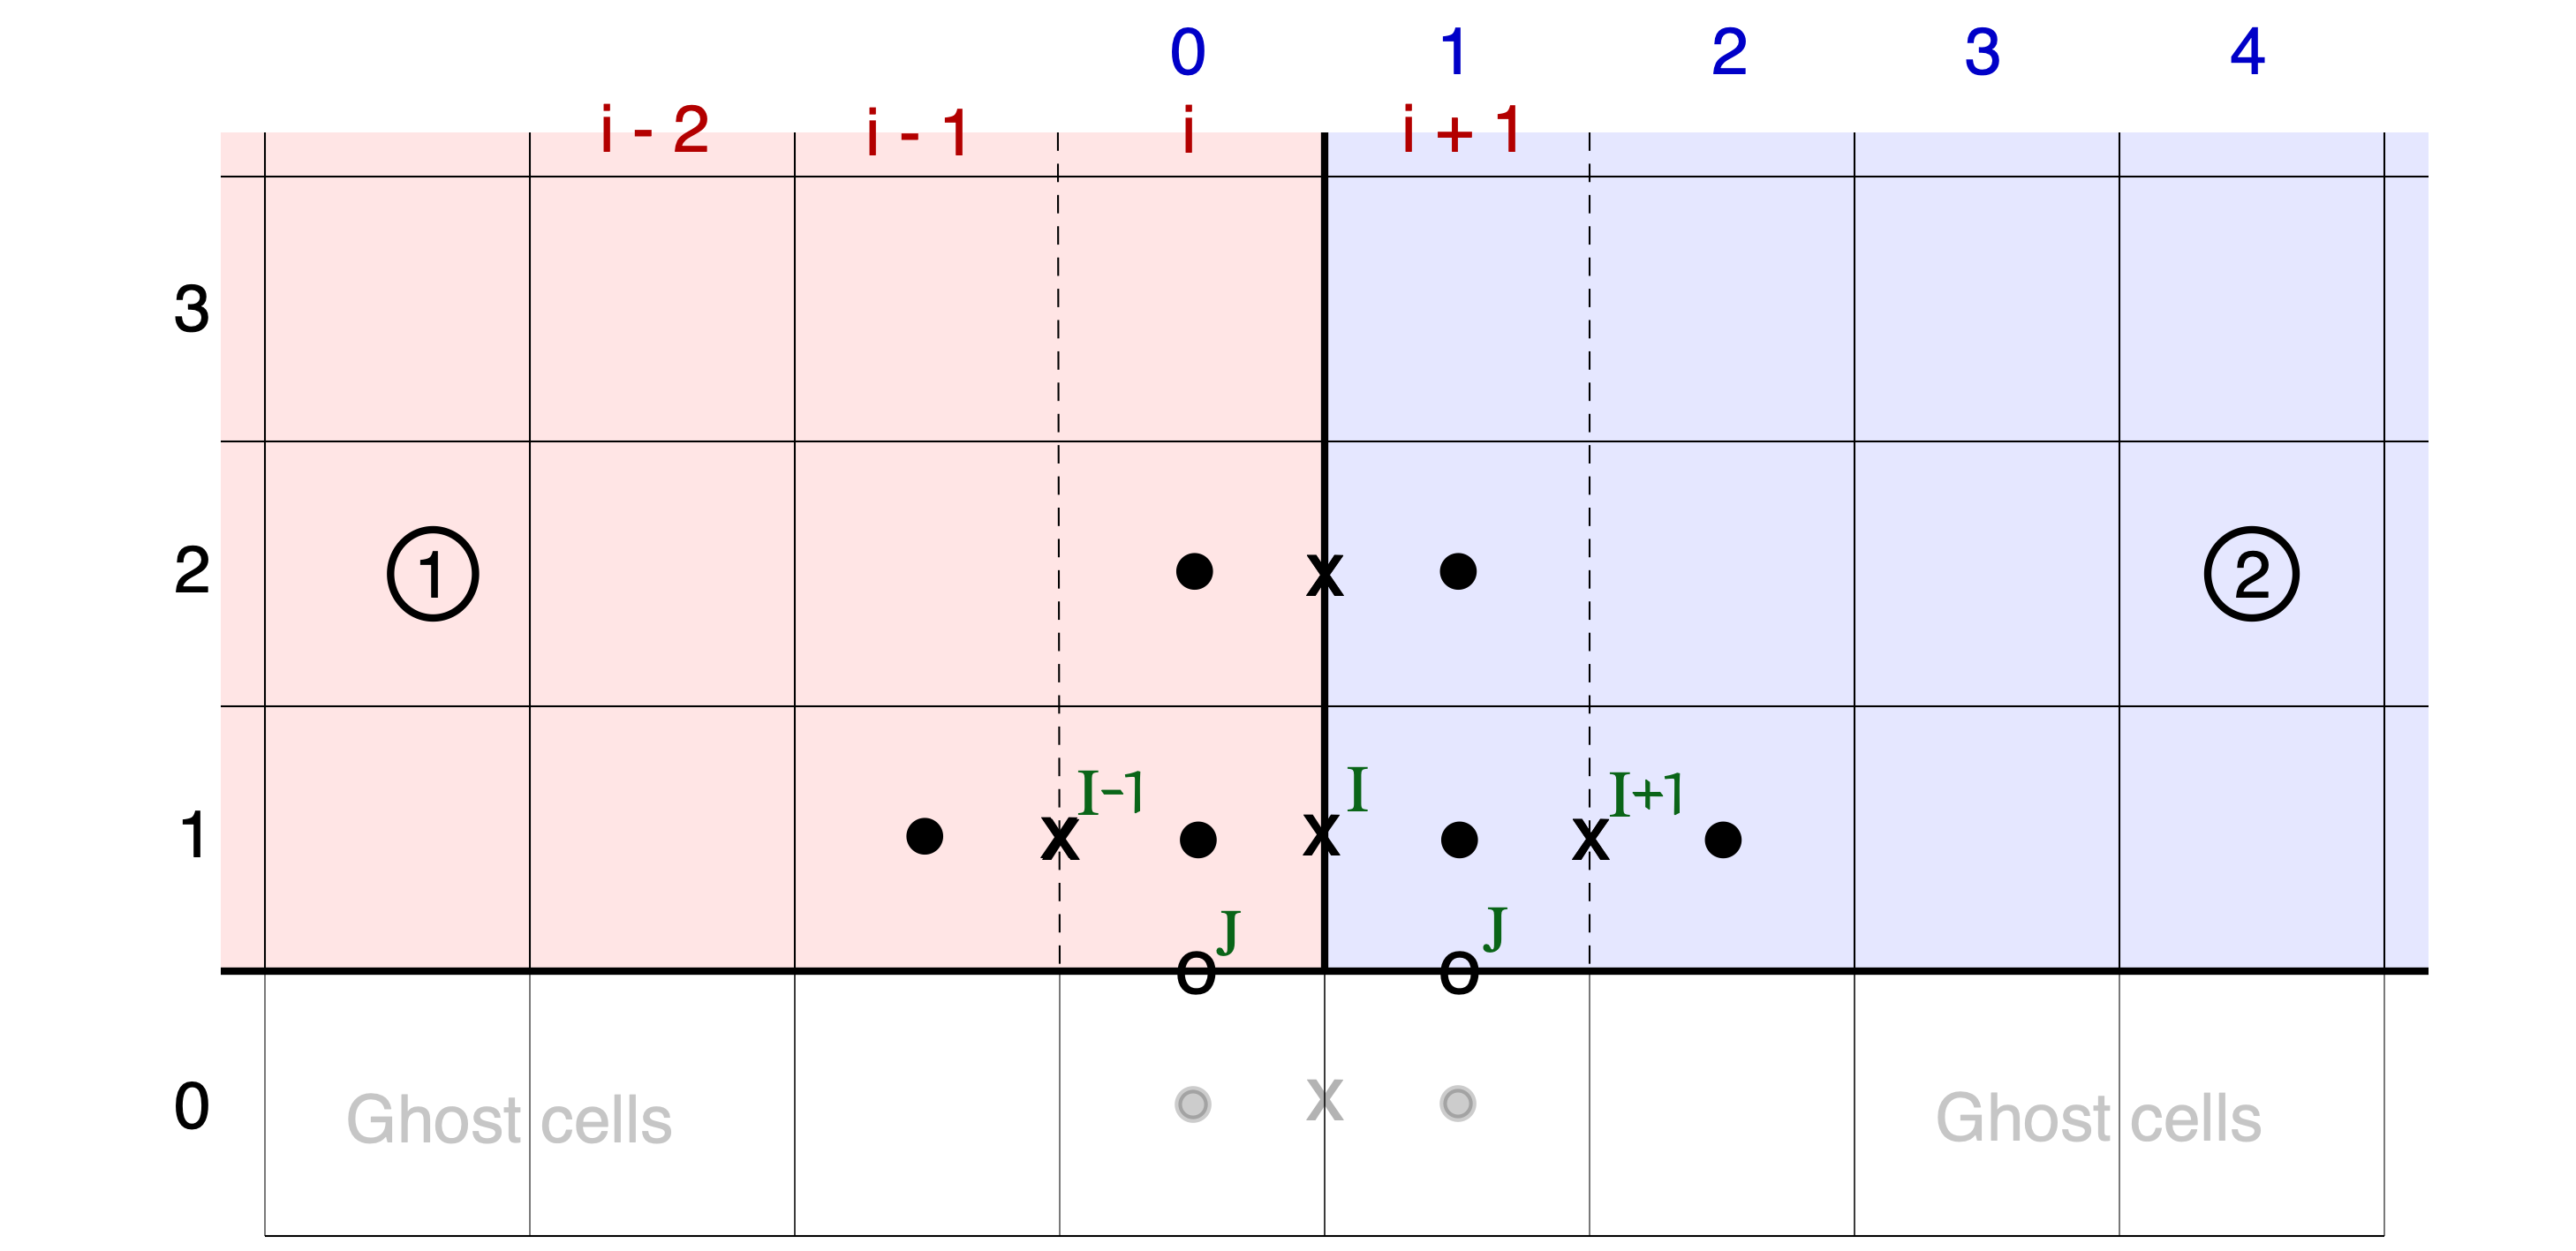
\includegraphics[width=14cm]{\figPath/MGM_Boundary.png}
\end{center}
\caption{Interface meets an external boundary}
\label{FIG_InterfaceBdry}
\end{figure}

%\noindent For the corresponding stencil in an interface node adjacent to the external boundary it holds
%\begin{align}  
%\HBO{I,1} &=  \left[\frac{\HBO{I-1,1} + \HBO{I+1,1}}{\DXT}  +  \frac{\HBO{I,0}  + \HBO{I,2}}{\DYT}\right] \biggl/ \left[\frac{2 }{\DXT}  +  \frac{2 }{\DYT}\right] \nonumber  
%\end{align}

\noindent The usual stencil in point $(I,1)$ looks like 
\[ \frac{\HBO{I-1,1} - 2 \HBO{I,1} + \HBO{I+1,1}}{\DXT}  +  \frac{\HBO{I,0} - 2 \HBO{I,1} + \HBO{I,2}}{\DYT} = 0\]


\subsubsection{Dirichlet case}

\noindent  The Dirichlet boundary values in the lower $y$-direction are defined as
\[\HBO{I,0}  = 2 \HBO{I,J} - \HBO{I,1} \qquad \rightarrow \qquad  \HBO{I,0}  =  - \HBO{I,1} \]
\noindent because $\HBO{I,J}=0$ due to the homogeneous Laplace boundary.
\noindent Thus, the stencil in $\HBO{I,1}$ looks like
\[\frac{\HBO{I-1,1} - 2 \HBO{I,1} + \HBO{I+1,1}}{\DXT}  +  \frac{ {\color{red}{-\HBO{I,1}}} - 2 \HBO{I,1} + \HBO{I,2}}{\DYT} = 0 \]
\noindent which results in  
\[\HBO{I,1} =  \left[\frac{\HBO{I-1,1} + \HBO{I+1,1}}{\DXT}  +  \frac{\HBO{I,2}}{\DYT}\right] \biggl/ \left[\frac{2 }{\DXT}  +  \frac{3}{\DYT}\right]\]

\newpage
\subsubsection{Neumann case}

\noindent  The Neumann boundary values in the lower $y$-direction are defined as
\[\frac{\HBO{I,0} - \HBO{I,1}}{\DY}  = 0   \qquad \rightarrow \qquad   \HBO{I,0} = \HBO{I,1} \]
\noindent Thus, the stencil in $\HBO{I,1}$ looks like
\[\frac{\HBO{I-1,1} - 2 \HBO{I,1} + \HBO{I+1,1}}{\DXT}  +  \frac{ {\color{red}{\HBO{I,1}}} - 2 \HBO{I,1} + \HBO{I,2}}{\DYT} = 0 \]
\noindent which results in  
\[\HBO{I,1} =  \left[\frac{\HBO{I-1,1} + \HBO{I+1,1}}{\DXT}  +  \frac{\HBO{I,2}}{\DYT}\right] \biggl/ \left[\frac{2 }{\DXT}  +  \frac{1}{\DYT}\right]\]


\subsection{Multiple meshes meet}
\noindent We still have to think of the treatment of cases where multiple meshes meet together. Please have a look at the node in the yellow mesh 4 which is not available by the usual WALL(IW) structures on mesh 1. Here, I think, we should use an alternative treatment or exchange the related values by a global data exchange (which would be possible, but would cost this exchange).

\begin{figure}[H]
\begin{center}
\includegraphics[width=12cm]{\figPath/mgm4.png}
\end{center}
\caption{Interfaces in case of 4 adjacent meshes}
\label{FIG_InterfaceFour}
\end{figure}

\begin{align}  
\HBO{I,j} &=  \left[\frac{\HBO{I-1,j} + \HBO{I+1,j}}{\DXT}  +  \frac{\HBO{I,j-1}  + \HBO{I,j+1}}{\DYT}\right] \biggl/ \left[\frac{2 }{\DXT}  +  \frac{2 }{\DYT}\right] \nonumber  
\end{align}
\noindent with

\begin{align}  
\HBO{I-1,j}  &= \frac{1}{2} (\HL{i-1,j}{1}{n-1} + \HL{i,j}{1}{n-1})  \nonumber \\[2ex]
\HBO{I+1,j} &= \frac{1}{2} (\HL{1,j}{2}{n-1} + \HL{2,j}{2}{n-1}) \nonumber \\[2ex]
\HBO{I,j+1} &= \frac{1}{2} (\HL{i,j+1}{1}{n-1} + \HL{1,j+1}{2}{n-1}) \nonumber \\[2ex]
\HBO{I,j-1} &= \color{red} {\frac{1}{2} (\HL{i,k}{3}{n-1} + \HL{1,m}{4}{n-1})} \nonumber \\[2ex]
\end{align}  



